\section{Security Model and Naming Convention}

\begin{figure*}[t]
  \centering
  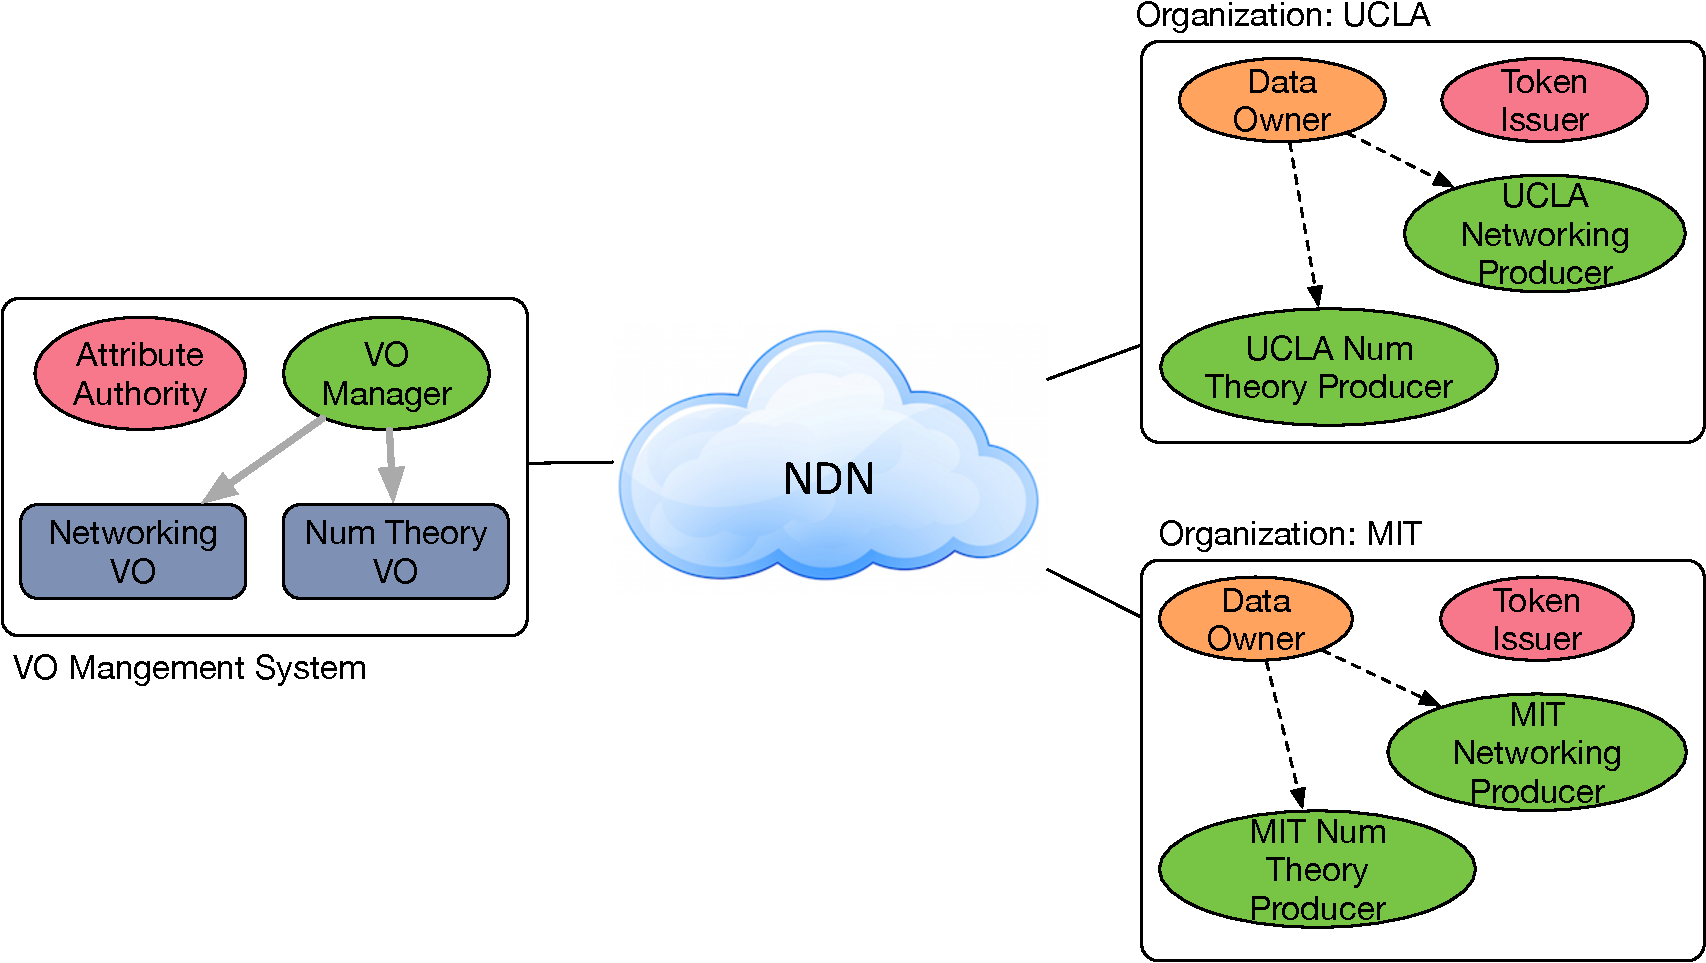
\includegraphics[scale=0.5]{figures/example}
  \vspace{-3mm}
  \caption{An example of how VO system work}
  \label{fig:example}
\end{figure*}

To facilitate explanation, in this paper, we will use the following example (\ref{fig:example}) to illustrate the security design and VO system.
There are two real-world organizations in our example: UCLA and MIT.
Both UCLA and MIT will produce networking lecture data and Number-theory lecture data.
Besides producers which are the green circles, each organization also contains one \textbf{data owner} and one \textbf{token issuer}.
Data owner is the one who define the access rules for producer.
Token issuer takes the duty to help attribute authority to verify consumer's identity.
Consumers should belongs to real organizations.

In NDN, each party is supposed to have an identity.
To make the example clear, we have the name like:

\begin{verbatim}
VO attribute authority: /vo/authority
VO manager: /vo/manager

UCLA token issuer: /ucla/token-issuer
UCLA network producer: /ucla/network
UCLA number theory producer: /ucla/num-theory
\end{verbatim}

\subsection{Ciphertext-policy Attribute-based Encryption over NDN}

There are usually three parties in CPABE: attribute authority (AA), producer and consumer.
The attribute authority would generate the secret master key and public parameters.
Producer would use the attribute policy, which is a string, to do the encryption and the consumer with sufficient decryption key could decrypt the content.
In our VO system, the AA would be deployed in VO management system while the producer will managed by the organization.

\subsubsection{Adopt AES to Handle Input with Unlimited Size}
Like RSA, the CPABE has limit input size and thus it is not viable for us to directly use CPABE to encrypt the content.
Therefore, we adopt AES and CBC to do the symmetric encryption to the input plaintext and use CPABE to only encrypt AES key, whose size is constant and short.
With AES, the system could be able to handle any size of input.

Therefore, inside each data packet, the content mainly contains two parts:
\begin{itemize}
\item Encrypted AES key. The AES key is encrypted by the attribute policy.
\item Encrypted content. The content is encrypted by the AES key.
\end{itemize}
When consumer fetches data back, the authorized consumer should first decrypt the AES key and use the AES key to decrypt content.
The format of the ciphertext is showed in \ref{fig:ciphertext}

\begin{figure}[H]
  \centering
  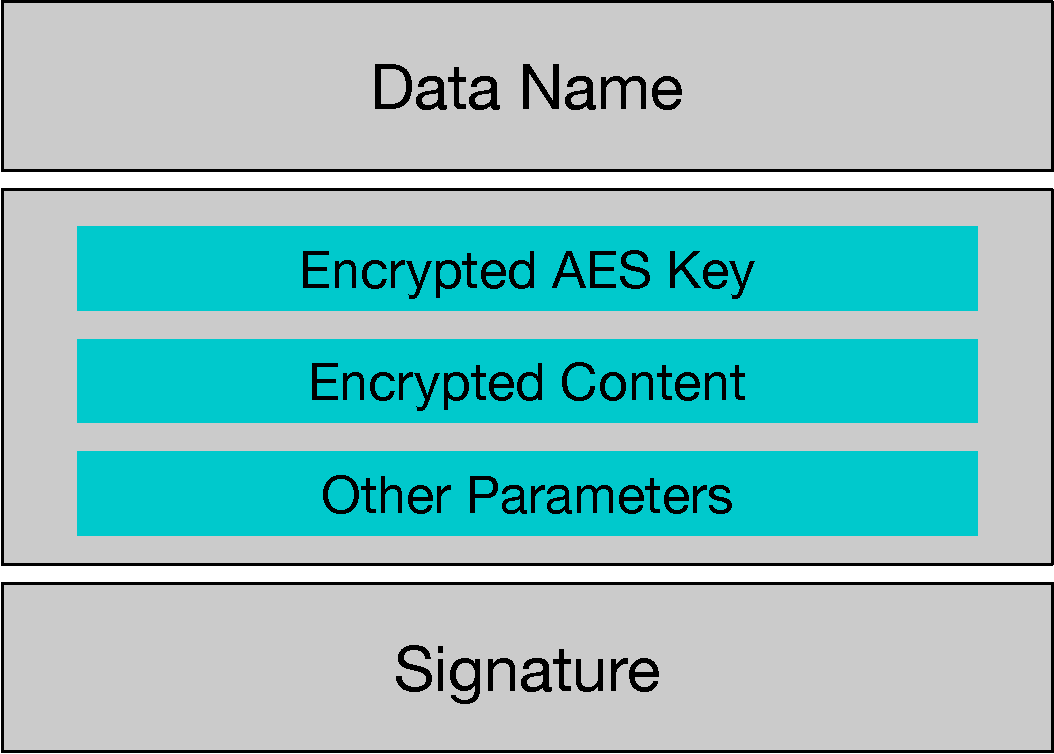
\includegraphics[width=0.3\textwidth]{figures/ciphertext}
  \vspace{-3mm}
  \caption{The format of ciphertext}
  \label{fig:token}
\end{figure}

\subsubsection{Separate Producer to Producer and Data Owner}
In practice, the data producer and the data owner may not be in the same devices.
For instance, in IOT environment, a smarthome controller may control all the smarthome devices like temperature sensors and AC in the room.
In this case, the controller controls multiple data producer and we consider the controller as \textit{data owner} and consider those devices who produce content as \textit{producer}.
Data owner itself doesn't produce content but it can command producers.
This kind of separation could improve the flexibility and let the controller to easily control the data it owns.

To achieve the similar separation in VO system, we introduce the data owner who can define the attribute policy for each producer.
For example, the data owner at UCLA could define the attribute rules \texttt{("professor'' OR "faculty") AND ucla} for the producer who produces networking lesson data.
In this way, only UCLA professors or faculty members could be able to consume the data.
Regarding the distribution of attribute policy, we let the data owner to send \textbf{signed interest} to producers whenever needed.
The signed interest is a special interest packet which also carries a signature from requester.
When receive policy signed interests, the producer must first verify the signature and make sure the command is from data owner.
After that, the producer can make the change and producer data under the new policy.

\subsubsection{Separate Attribute Authority to Attribute Authority and Token Issuer}
It is simple to know that, the central attribute authority needs to issue decryption key to consumers.
This means the authority itself needs to remember consumer's identity.
However, this logic is not viable in large scale: in our example, the attribute authority needs to remember all the consumers from both UCLA and MIT.
It has neither good privacy for student's information nor good efficiency for the attribute authority have high overload.

To mitigate the issue, we separate the attribute authority to one attribute authority who issue the crypto decryption key and multiple token issuers who verify consumer's identity.
Each member organization should have one token issuer.
The privacy can be ensured for organization will take it's own business to verify their consumers and the information of consumers won't go to the third party.
Also, this design saves attribute authority's resources.
The only cost is for attribute authority to build up the trust to each token issuer.

\begin{figure}[H]
  \centering
  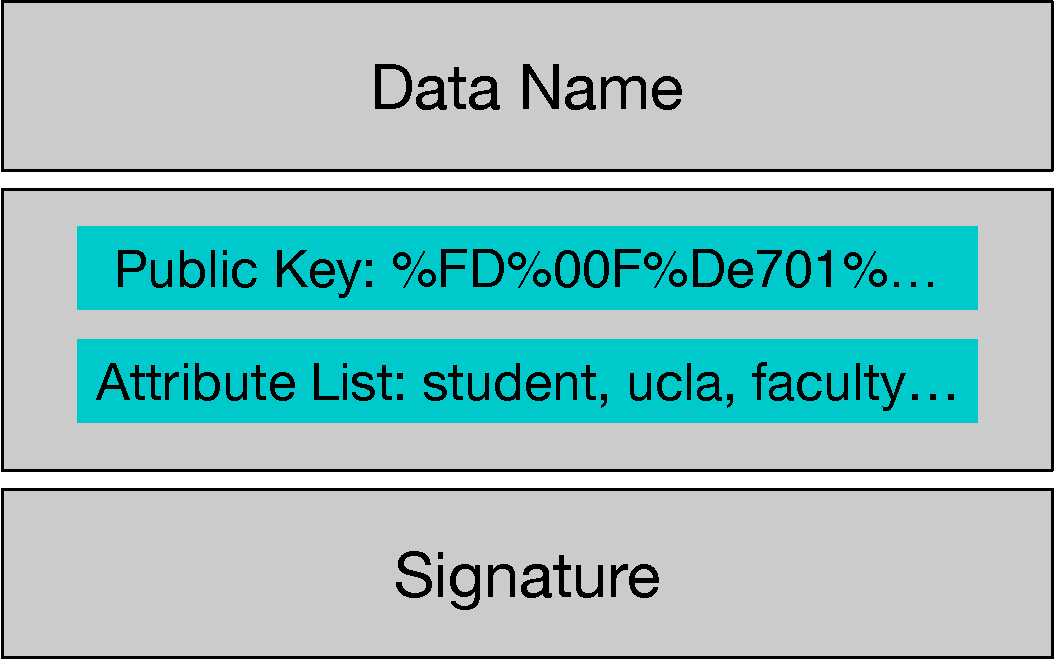
\includegraphics[width=0.3\textwidth]{figures/token}
  \vspace{-3mm}
  \caption{The format of token}
  \label{fig:token}
\end{figure}

To implement the separation, after token issuer's verifying consumer's access rights, the token issuer would issue a token, which contains consumer's public key bits and a list of attributes.
The format of the token is like \ref{fig:token}
Also, the data packet carries the token will also be signed by token issuer.
Token issuer can then use the token to get the decryption key for consumer from AA.
Notice even though the key would be fetch by token issuer, token issuer cannot get the key for the key would be encrypted by consumer's public key (AA get the public key from token).

\subsection{Naming Convention}

To facilitate the use of NDN, we have the naming convention to simplify the whole system.

\subsubsection{Data Name Carries Attribute Policy}

In our system, the naming convention of data packet is like:
\begin{figure}[H]
  \centering
  
\includegraphics[width=0.5\textwidth]{figures/data-name}
  \vspace{-3mm}
  \caption{Data packet naming convention}
\end{figure}
For instance, to produce data only for UCLA's professors, the producer \ndnName{/ucla/network} should use the policy \ndnName{professor AND ucla} to do the encryption.
A possible name can be like: \ndnName{/ucla/network/cs118-lesson1/''professor AND ucla''}.
One benefit is that the consumer can easily know whether his/her decryption is sufficient or not to decrypt the content.

\subsubsection{Signed Interest Carries Attribute Policy}

In NDN, it's difficult for a host to actively send out a data packet while it's easy to send out interest.
In our system, we let data owner send out signed interest to command each producer.
The naming convention of attribute policy command interest is like:

\begin{figure}[H]
  \centering
  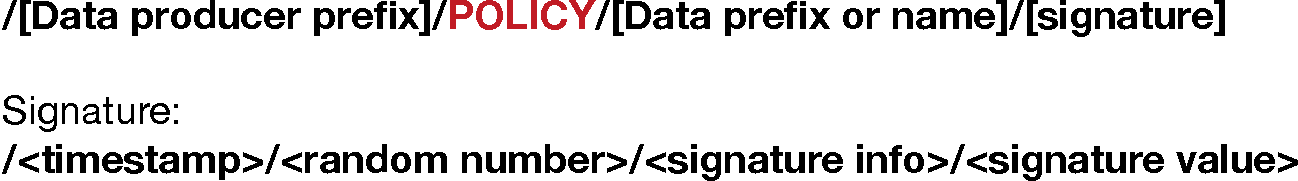
\includegraphics[width=0.5\textwidth]{figures/policy-interest}
  \vspace{-3mm}
  \caption{Policy interest naming convention}
\end{figure}

For example, if the UCLA data owner wants to command the producer \ndnName{/ucla/num-theory} that all the data under the prefix \ndnName{/lesson1} should have the policy \ndnName{students AND (ucla or mit)}.
In this case, the command interest would be like:
\ndnName{/ucla/num-theory/POLICY/lesson1/[signature]}.
Once get the command from token issuer, the producer will first check the signature.
If the interest can be trusted, the producer should follow the command.

\subsubsection{Signed Interest Carries Token}

Similar as the previous design, to make sure the security communication between token issuer and AA, we let the token issuer to send interest carrying the token to AA.
The naming convention for this kind of  interest is like:

\begin{figure}[H]
  \centering
  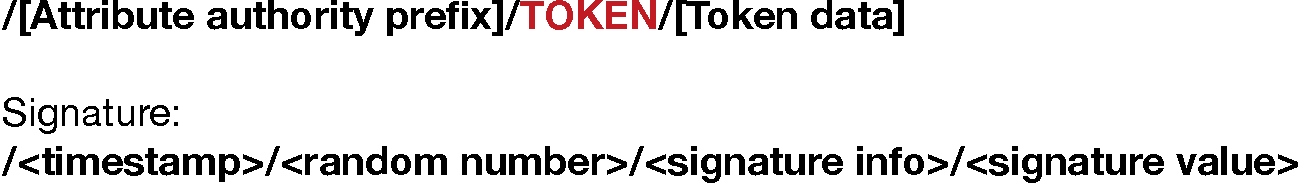
\includegraphics[width=0.5\textwidth]{figures/token-interest}
  \vspace{-3mm}
  \caption{Token interest naming convention}
\end{figure}

This naming convention somehow abuse the interest to pass data content but it only happens during the preliminary phase and it does not hurt.
Notice the interest is not a signed interest for there is already a signature inside the token.
Because the replied data's content is encrypted by consumer's public key, no one except the consumer can get the key: it is secure to send back the data publicly.

\subsection{Access Model}
\subsubsection{Setup}
In the setup phase, the attribute authority would first generate CPABE public parameters and master key.
Public parameters would be wrapped into a data packet and be signed by VO management system.
The master key should be carefully kept by AA.
After the that, the AA should publish the public parameter data packet.
To improve the efficiency, the data packet can be cached in some in-network storage system or be cached by network infrastructure like routers and switches.

Notice every party in the system should fetch the public parameters packet.
Once the signature is verified, the public parameters should be kept by each party until the public parameters expires.

\subsubsection{Key Generation}
In this phase, the token issuer should verify consumers belonging to their own organizations and generate tokens for consumers.
The token issuer should then express the tokens to AA and ask AA to generate the decryption keys and fetch the keys back.
Whenever the AA receives the token, AA must verify the token's signature first.
After that, the AA could use the master key and the attribute list to generate the decryption key.
Then the decryption key should be encrypted by the public key recorded in the token.

\subsubsection{Encryption}
Whenever a party wants to become a producer (and a data owner), it can immediately define the attribute policy and start producing content.
As long as the host has the public parameter, there is no requirements for it to become a producer.
The attribute policy is only a string containing the attribute and the logic gates.

\subsubsection{Decryption}
Once the consumer gets the decryption key, the consumer then has a set of attributes.
Consumer can decide whether he/she is allowed to consume the content by checking the data name.
If the consumer's attributes is sufficient, the consumer could use the key to decrypt the AES key first and then decrypt the content with the AES key.